% Figure JEn2026-01: a play of Cops and Robbers. A moving token leaves a dashed copy
% at its previous vertex, and a straight arrow beside the edge shows the move. Top row: one cop on a tree; the robber
% is cornered at a leaf and captured. Bottom row: one cop on C_4; the robber keeps
% distance two indefinitely. Requires only the tikz core (arrow tip "stealth").
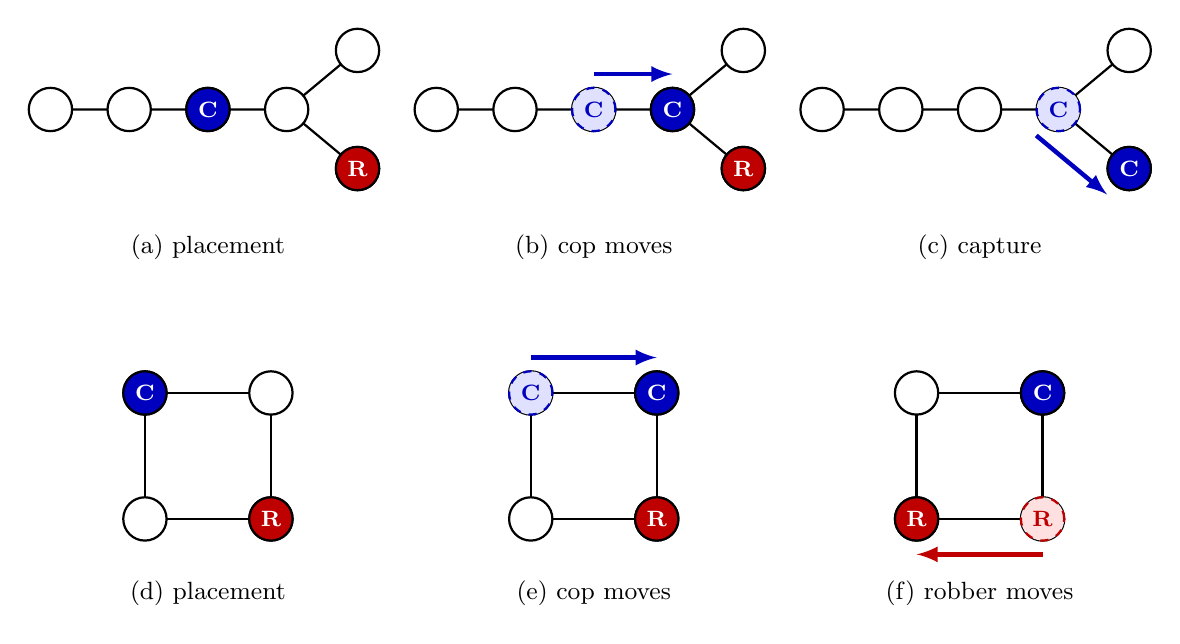
\begin{tikzpicture}[>=latex,
  vertex/.style={circle,draw,thick,fill=white,minimum size=5.5mm,inner sep=0pt},
  cop/.style={vertex,fill=blue!75!black,text=white,font=\bfseries\footnotesize},
  robber/.style={vertex,fill=red!75!black,text=white,font=\bfseries\footnotesize},
  ghostcop/.style={vertex,draw=blue!75!black,dashed,fill=blue!12,text=blue!75!black,font=\bfseries\footnotesize},
  ghostrob/.style={vertex,draw=red!75!black,dashed,fill=red!12,text=red!75!black,font=\bfseries\footnotesize},
  cmove/.style={->,line width=1.6pt,blue!75!black},
  rmove/.style={->,line width=1.6pt,red!75!black},
  lab/.style={font=\small},
  tree/.pic={
    \draw[thick] (-2,0)--(1,0) (1,0)--(1.9,0.75) (1,0)--(1.9,-0.75);
    \foreach \p in {(-2,0),(-1,0),(0,0),(1,0),(1.9,0.75),(1.9,-0.75)}
      \node[vertex] at \p {};
  },
  square/.pic={
    \draw[thick] (-0.8,-0.8) rectangle (0.8,0.8);
    \foreach \p in {(-0.8,-0.8),(0.8,-0.8),(0.8,0.8),(-0.8,0.8)}
      \node[vertex] at \p {};
  }]
% ---- top row: a tree ----
\begin{scope}[xshift=0cm]
  \pic {tree};
  \node[cop] at (0,0) {C};
  \node[robber] at (1.9,-0.75) {R};
  \node[lab] at (0,-1.75) {(a) placement};
\end{scope}
\begin{scope}[xshift=4.9cm]
  \pic {tree};
  \node[ghostcop] at (0,0) {C};
  \node[cop] at (1,0) {C};
  \node[robber] at (1.9,-0.75) {R};
  \draw[cmove] (0,0.45) -- (1,0.45);
  \node[lab] at (0,-1.75) {(b) cop moves};
\end{scope}
\begin{scope}[xshift=9.8cm]
  \pic {tree};
  \node[ghostcop] at (1,0) {C};
  \node[cop] at (1.9,-0.75) {C};
  \draw[cmove] (0.72,-0.33) -- (1.62,-1.08);
  \node[lab] at (0,-1.75) {(c) capture};
\end{scope}
% ---- bottom row: the cycle C_4 ----
\begin{scope}[yshift=-4.4cm,xshift=0cm]
  \pic {square};
  \node[cop] at (-0.8,0.8) {C};
  \node[robber] at (0.8,-0.8) {R};
  \node[lab] at (0,-1.75) {(d) placement};
\end{scope}
\begin{scope}[yshift=-4.4cm,xshift=4.9cm]
  \pic {square};
  \node[ghostcop] at (-0.8,0.8) {C};
  \node[cop] at (0.8,0.8) {C};
  \node[robber] at (0.8,-0.8) {R};
  \draw[cmove] (-0.8,1.25) -- (0.8,1.25);
  \node[lab] at (0,-1.75) {(e) cop moves};
\end{scope}
\begin{scope}[yshift=-4.4cm,xshift=9.8cm]
  \pic {square};
  \node[cop] at (0.8,0.8) {C};
  \node[ghostrob] at (0.8,-0.8) {R};
  \node[robber] at (-0.8,-0.8) {R};
  \draw[rmove] (0.8,-1.25) -- (-0.8,-1.25);
  \node[lab] at (0,-1.75) {(f) robber moves};
\end{scope}
\end{tikzpicture}